\begin{figure}
    \centering
    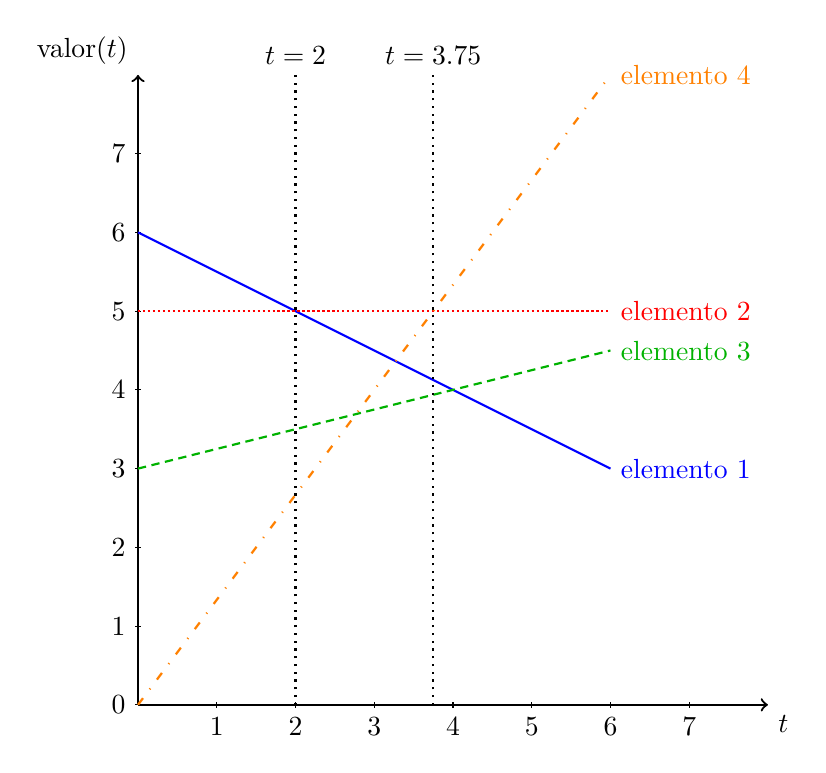
\begin{tikzpicture}
        % \draw[step=1cm,lightgray,very thin] (-2,-2) grid (10,10);
        \draw[thick,->] (0,0) -- (8,0)
            node[anchor=north west] {$t$};
        \draw[thick,->] (0,0) -- (0,8)
            node[anchor=south east] {valor$(t)$};
        \foreach \x in {1, 2,..., 7}
            \draw (\x cm,1pt) -- (\x cm,-1pt)
                node[anchor=north] {$\x$};
        \foreach \y in {0, 1, ..., 7}
            \draw (1pt,\y cm) -- (-1pt,\y cm)
                node[anchor=east] {$\y$};
        \draw[solid, thick, color=blue]
            (0, 6) -- (6, 3) node[anchor=west] {elemento 1};
        \draw[densely dotted, thick, color=red]
            (0, 5) -- (6, 5) node[anchor=west] {elemento 2};
        \draw[densely dashed, thick, color=black!30!green]
            (0, 3) -- (6, 4.5) node[anchor=west] {elemento 3};
        \draw[loosely dashdotted, thick, color=orange]
            (0, 0) -- (6, 8) node[anchor=west] {elemento 4};
        \draw[dotted, thick, color=black]
            (2, 0) -- (2, 8) node[anchor=south] {$t = 2$};
        \draw[dotted, thick, color=black]
            (3.75, 0) -- (3.75, 8) node[anchor=south] {$t = 3.75$};
    \end{tikzpicture}
    \caption[Exemplo máximo cinético]{O maior valor até o instante
    $t = 2$ é o do elemento $1$. Em seguida, o maior valor passa a
    ser o do elemento $2$ até o instante $t =3.75$, que é quando o
    elemento $4$ passa a superar todos os outros.}
    \label{fig:max:example}
\end{figure}